\begin{figure}[!p] %s state preferences regarding figure placement here

% use to correct figure counter if necessary
%\renewcommand{\thefigure}{2}

\centering
\subfigure[URL reference]{%
\label{fig:verification-a}%
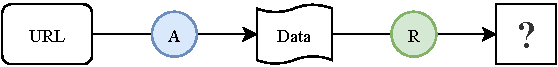
\includegraphics[scale=0.74, right]{figures/fig4a.pdf}} \\
\subfigure[URL reference with content hash]{%
\label{fig:verification-b}%
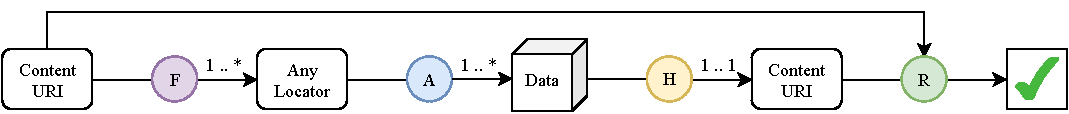
\includegraphics[scale=0.74, right]{figures/fig4b.pdf}} \\
\subfigure[Content URI reference]{%
\label{fig:verification-c}%
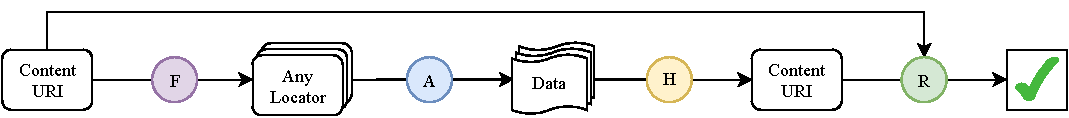
\includegraphics[scale=0.74, right]{figures/fig4c.pdf}} \\
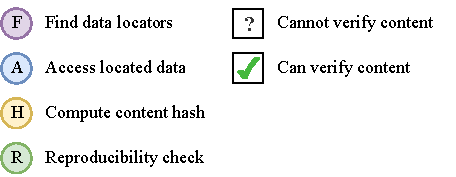
\includegraphics[scale=.9]{figures/fig4legend.pdf}%

\caption{Content resolution and verification for references that use location- versus content-based identifiers. \subref{fig:verification-a} Location-based identifiers (e.g. URLs) cannot verify the authenticity of retrieved content and are vulnerable to link rot due to the use of a fixed locator. \subref{fig:verification-b} If the content hash of the referenced data is known, the authenticity of retrieved data can be verified by comparing the hash of the retrieved data with the provided content hash. However, the fixed locator is still vulnerable to link rot. \subref{fig:verification-c} Content-based identifiers (e.g. Content URIs) can be used to find several locators for the referenced data and contain a content hash to verify the authenticity of retrieved data. The decoupling of the reference from a fixed locator makes the reference resistant to link rot.
}%

\label{fig:verification} % \label works only AFTER \caption within figure environment

\end{figure}
